\documentclass[12pt]{article}
\usepackage{amsmath}
\usepackage{graphicx}
\usepackage{float}
\usepackage{caption}
\usepackage{subcaption}
\usepackage[margin=1in]{geometry}

\title{ELCT 562 PA3}
\author{J. Vaught}
\date{\today}

\begin{document}

\maketitle

\section{Introduction}
In wireless communication systems, the quality and reliability of a signal transmission depend significantly on the channel characteristics. Two critical parameters for characterizing the wireless channels are coherence bandwidth (BW) and coherence time.

\subsection{Coherence Bandwidth}
Coherence bandwidth is a measure of the range of frequencies over which the channel can be considered "flat". In other words, it is the range of frequencies over which the channel has a constant gain and linear phase response. It is inversely related to the multipath spread of the channel: a wide multipath spread results in a small coherence bandwidth.

\subsection{Coherence Time}
Coherence time is the time duration over which the channel impulse response is considered invariant. During this time, the channel can be assumed to be static and unchanging. Coherence time is inversely proportional to the Doppler spread, which is affected by the relative motion between the transmitter and receiver.
\newpage
\section{Communication Scenarios and Analysis}
The coherence time and bandwidth for different communication scenarios are analyzed based on the environmental and mobility factors.

\subsection{Scenario A}
In an office environment without a Line of Sight (LoS) path, two stationary laptops communicate through a complex channel characterized by multiple signal reflections, diffractions, and scattering. The coherence time is relatively high because the environment is static, and the channel characteristics do not change quickly over time. Objects in the office, such as furniture and walls, remain fixed, providing a consistent pattern of multipath components. On the other hand, the coherence bandwidth is expected to be lower. This is because the multipath effects caused by the office environment lead to different path lengths that the signal can travel, causing a spread in the delay of received signal components. Such a scenario induces a frequency-selective fading effect, where different frequencies of the signal experience different levels of attenuation and phase shifts, hence a reduced coherence bandwidth.

\begin{figure}[htbp]
\centering

\includegraphics[width=\textwidth]{a.png}
\caption{Coherence Time and Bandwidth for Stationary Laptops (No LoS)}
\end{figure}

\newpage
\subsection{Scenario B}
When two cars are approaching each other at high speeds, the communication channel between them is dominated by a strong LoS component. The relative velocity between the cars introduces a significant Doppler effect, which reduces the coherence time of the channel. The Doppler spread, which is proportional to the relative speed, causes the channel characteristics to vary more rapidly over time. However, the strong LoS contributes to a flat fading channel where the signal experiences uniform fading across the bandwidth. Thus, the coherence bandwidth is relatively high as the multipath effects are minimal, and the channel's frequency response remains flat over a wider frequency range.

\begin{figure}[htbp]
\centering

\includegraphics[width=\textwidth]{b.png}
\caption{Coherence Time and Bandwidth for Approaching Cars (Strong LoS)}
\end{figure}

\newpage
\subsection{Scenario C}
Satellite communication channels are characterized by a predominantly free-space path with minimal obstructions, leading to minimal multipath fading and a flat channel response over a wide frequency range. This results in a high coherence bandwidth. Additionally, since satellites are in a stable orbit with a constant relative distance to each other, the channel impulse response remains nearly static over long periods. This stability grants the system a very high coherence time, as the lack of significant relative motion between the satellites means the Doppler spread is negligible. Consequently, the communication channel remains coherent for longer durations, and the channel's properties change very slowly.

\begin{figure}[htbp]
\centering
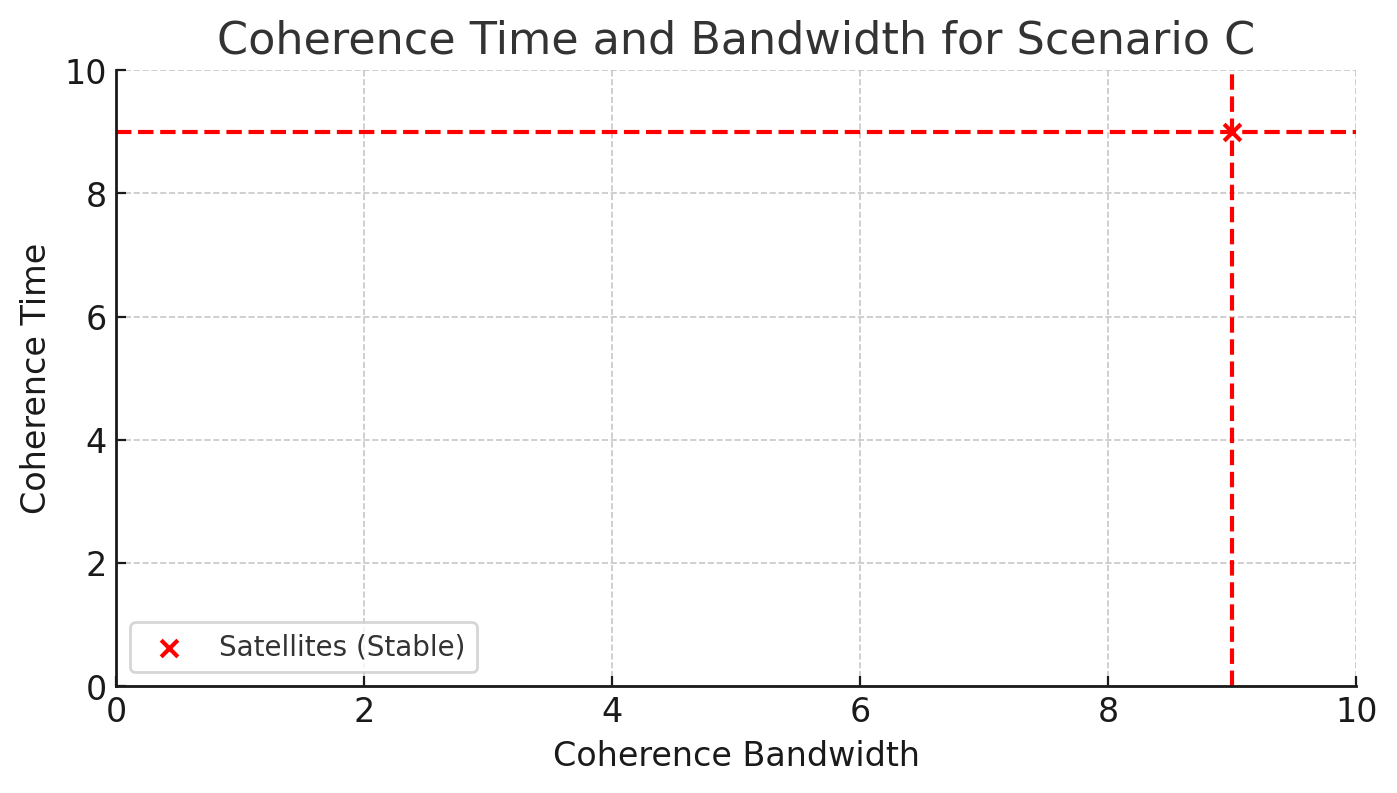
\includegraphics[width=\textwidth]{c.png}
\caption{Coherence Time and Bandwidth for Satellites (Stable)}
\end{figure}

\newpage
\subsection{Scenario D}
Racing drones in a dense forest present a highly dynamic and challenging communication environment. The high-speed movement of the drones and the constantly changing obstacles (such as trees and foliage) that block the LoS path create a rapidly varying multipath scenario. This results in a low coherence time due to the high Doppler spread and frequent changes in the channel's impulse response. Furthermore, the multiple scattering points in the forest cause the signal to take various paths with different lengths to reach the receiver, inducing significant delay spread. This environment leads to a frequency-selective fading channel where the coherence bandwidth is also low, as different frequency components of the signal are affected differently by the channel, causing distortion over a narrow frequency range.

\begin{figure}[htbp]
\centering
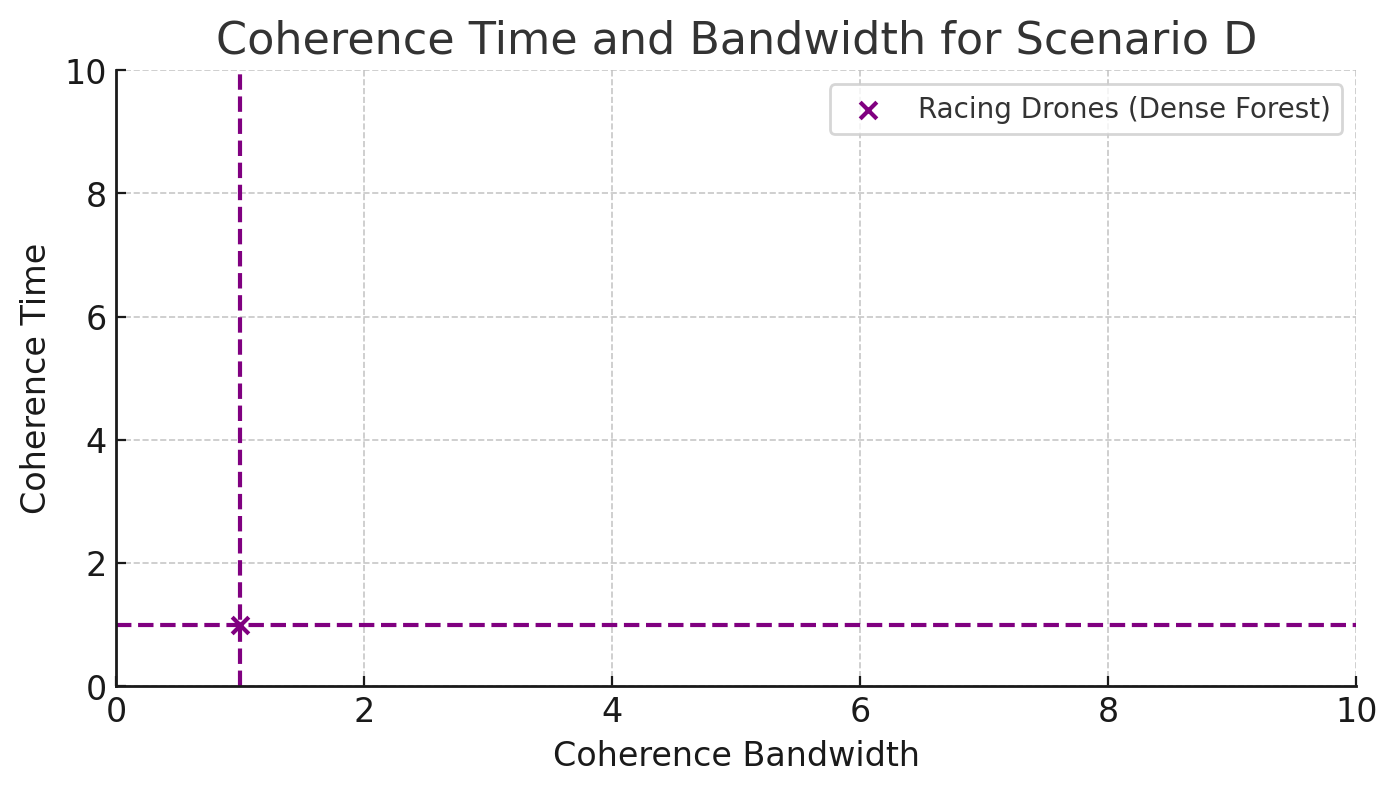
\includegraphics[width=\textwidth]{d.png}
\caption{Coherence Time and Bandwidth for Racing Drones (Dense Forest)}
\end{figure}


\end{document}
